\documentclass[a4paper]{article}

% Font stuff
\usepackage{fouriernc}
%\usepackage{mathptmx}
\usepackage[T1]{fontenc}

% Extra math symbols
\usepackage{amsmath}
\usepackage{amssymb}
\usepackage{amsthm}

% IEEE equation array
\usepackage[retainorgcmds]{IEEEtrantools}

% bibliography
%\usepackage[square]{natbib}

% adds a toc to the pdf file, and makes refs clickable
\usepackage[bookmarks,colorlinks=true]{hyperref}

% for \llbracket, \rrbracket (scott brackets)
% Needs debian package texlive-math-extra
\usepackage{stmaryrd}

% proof trees
\usepackage{bussproofs}
\def\defaultHypSeparation{\hskip .1in}

% tikz drawing library
\usepackage{tikz}
\usetikzlibrary{positioning}
\usetikzlibrary{matrix}
\usetikzlibrary{arrows}

% === BEGIN custom commands

\newcommand{\arr}{\rightarrow}
\newcommand{\todo}[1]{\bigskip \noindent \emph{todo: #1}}
%\newcommand{\todo}[1]{}
\newcommand{\semantics}[1]{\llbracket #1 \rrbracket}

% church-style (explicit) abstraction. We adjust the spacing around the colon and dot
\newcommand{\church}[4]{#1 #2\!:\!#3\,.\,#4}

\newcommand{\curry}[3]{#1 #2\,.\,#3}

% something is of type something  x : A, we adjust the spacing
\newcommand{\oftype}[2]{#1\!:\!#2}

% === END custom commands

\begin{document}

\title{A Compiler for SPL, the Simple~Programming~Language}
\author{Markus Klinik (s4220315)}
\maketitle

\begin{abstract}

This report describes design decisions for the implementation of the compiler
for the course NWI-IMC004 Compiler Construction.

\end{abstract}

\section{Implementation language}

The SPL compiler is written in Haskell, because a functional language is
well-suited for the various programming tasks that arise when implementing a
compiler.

\begin{itemize}

  \item Traversing trees by pattern matching and recursion on algebraic
  data types is most convenient.

  \item Immutable data structures and sharing allow a style of
  programming that resembles mathematical definitions.  This comes in
  handy for example when an environment needs to be passed modified to
  a subcomputation, but the original environment is needed again later.

\end{itemize}

\section{Grammar}

The Parser is implemented in a top-down style using the uu-parsinglib
parser combinator library.  The grammar is kept mostly unmodified,
making use of the backtracking features of uu-parsinglib.  Focus was
put more on conciseness of the implementation rather than run-time
performance.

There are three important changes to the grammar.  The first one is the
introduction of intermediate non-terminals to account for the different
precedence levels of binary operators.  These intermediate
non-terminals are not given names, they arise by mapping parser
constructing functions over a suitably nested list of strings, followed
by folding the result with left- and right chaining combinators,
according to their associativity.

The second change to the grammar is one left-factorization in the rule
for expressions, to get rid of backtracking when an expression in the
input starts with many opening parenthesis.

The third grammar change is due to scoping issues, and described in section
\ref{sec:scopingRules}.

\section{Scoping rules}

Before getting to scoping rules, we need to discuss the role of type
annotations, and mutual recursion.

\subsection{Type annotations}

There are two different ways to interpret type
annotations \cite{Pierce2002a}.  Consider the following two lambda-terms, one
in Curry-style without type annotations and the other one in
Church-style with type annotations.

\begin{IEEEeqnarray}{c}
\label{curryterm}\curry{\lambda}{f}{\curry{\lambda}{x}{f(f x)}}\\
\label{churchterm}\church{\lambda}{f}{a}{\church{\lambda}{x}{b}{f(f x)}}
\end{IEEEeqnarray}

When type checking term (\ref{curryterm}) in a polymorphic type system,
the type inference algorithm would infer that the term has type
$(a \arr a) \arr a \arr a$, and conclude that the term is
well typed.  For term (\ref{churchterm}), considered under the same
typing rules, the question arises what the meaning of the type
variables $a$ and $b$ is.  These two are possible:

\begin{enumerate}

 \item \label{interp_exists} There exists a substitution ${}^*$ for
 $a$, $b$, $c$ such that term (\ref{churchterm}) has type $(a \arr b
 \arr c)^*$.

 \item \label{interp_forall} For all substitutions ${}^{*_1}$ of $a$
 and $b$, there exists a substitution ${}^{*_2}$ of $c$ such that term
 (\ref{churchterm}) has type $(a^{*_1} \arr b^{*_1} \arr c^{*_2})$.

\end{enumerate}

Under the first interpretation, term (\ref{churchterm}) would
be well-typed, because clearly such a substitution exists.  Take $[a
\arr (\text{Int} \arr \text{Int}), b \arr \text{Int}, c \arr
\text{Int}]$.

Under the second interpretation, term (\ref{churchterm}) would not be
well-typed, because for the substitution $[a \arr \text{Int}, b \arr
\text{Int}]$, there is no substitution ${}^*$ for $c$ such that the term has
type $(\text{Int} \arr \text{Int} \arr c^*)$.

A similar term that would be well-typed under both the first and the second
interpretation is the following one:

\begin{IEEEeqnarray*}{c}
\church{\lambda}{f}{a \arr a}{\church{\lambda}{x}{a}{f(f x)}}
\end{IEEEeqnarray*}

The grammar for SPL, as given in the first exercise, does not allow type
annotations of function types.  We therefore have to either choose the first
interpretation, or add function types to the grammar to choose the second
interpretation.  The first interpretation seemed more challenging, so the
present implementation of the SPL compiler chooses this one.

\subsection{Polymorphism and mutual recursion}

When inferring the type of a set of mutually recursive functions, all
constraints that arise in the bodies of the functions have to be unified
simultaneously.  Otherwise, the types of the functions become too general.
Consider the following mutually recursive functions $f$ and $g$.

\begin{verbatim}
a f(b x, c y) { return g(y, x); }
a g(b x, c y) { return f(x, y); }
\end{verbatim}

The type of both of them must be $\forall a b . (a \arr a \arr b)$, but if the
type inference algorithm would introduce $f$ all-quantified into the context
before calculating the constraints of $g$, it would infer the type $\forall a b
c .  (a \arr b \arr c)$ for both $f$ and $g$.

On the other hand, the constraints of functions which are not mutually recursive
must never be unified simultaneously, because otherwise they could get types
which are not general enough.  Consider the following example.

\begin{verbatim}
a id(a x) { return x; }
Void h() { id(10); return; }
\end{verbatim}

If the type inference algorithm would unify the types of \emph{h} and \emph{id}
simultaneously, it would infer the type $(\text{Int} \arr \text{Int})$ for
\emph{id}.  This means that the type inference algorithm must first infer the
type of \emph{id} separately, introduce it all-quantified as $\forall a . (a
\arr a)$ to the context, and then infer the type of \emph{h}.

It therefore seems that no matter which of the above we choose, the following
program would give either a type error for \emph{id} or too general types to
\emph{f} and \emph{g}.

\begin{verbatim}
a id(a x) { return x; }
a f(b x, c y) { id(10); return g(y, x); }
a g(b x, c y) { id(True); return f(x, y); }
\end{verbatim}

It appears that we must choose one of the following alternatives.

\begin{itemize}
  
  \item Forbid mutual recursion.

  \item Require forward declarations, like in C.

  \item Let the programmer explicitly specify the functions whose types should
  be unified simultaneously.

  \item Make the type checker analyse dependencies of function definitions to
  find cycles and thus automatically determine which functions to unify
  simultaneously.

\end{itemize}

The first alternative would result in a much easier implementation of the type
checker, at the cost of flexibility for the programmer.

The second alternative would run counter to the idea of type inference.

The third alternative, realizable for example by explicit let-bindings which
allow several bindings to be defined at once, places the burden of resolving
dependencies on the programmer.

Clearly, the fourth alternative would be preferable, and it should indeed be
possible to automatically determine dependencies between functions by just
looking at the free variables that occur in the function bodies.

The implementation at hand chooses the third alternative, as a tradeoff between
flexibility and ease of implementation.

\subsection{Polymorphism and assignments}

Another issue is polymorphic type inference in presence of assignments.  The
question is whether to all-quantify free type variables in local and global
variables.  To illustrate the problem, consider the following program.

\begin{verbatim}
fun f() {
  var x = [];
  x = 1:[];
  x = True:[];
}
\end{verbatim}

If the type checker would introduce $x$ all-quantified to the environment when
type checking the function body, $x$ would be of type $\forall a . [a]$, which
could be specialized to $[\text{Int}]$ in the first assignment, and to
$[\text{Bool}]$ in the second.  Clearly, this is unsound.  Pierce, in his
chapter about mutable references \cite{Pierce2002a}, solves this problem by
all-quantifying the type of an identifier only if its initializer is a syntactic
value.  He argues that this restriction has no big impact on usability.  In his
language, reference cell constructors are not values, so identifiers initialized
with a reference cell are never all-quantified.  In SPL, variables are always
mutable, every variable is therefore always implicitly a reference cell, so by
adopting the \emph{value restriction} in the type checker at hand, the types of
variables are never all-quantified.  This gives the desired type error for the
program above. Unfortunately this comes at the tradeoff that programs like the
following, in which an identifier is never assigned to, also give type errors.
This is because the type of $x$ gets constrained to both $[\text{Int}]$ and
$[\text{Bool}]$.

\begin{verbatim}
fun f() {
  var x = [];
  return (1:x, True:x);
}
\end{verbatim}

In the current implementation of the type checker for SPL, we adopt this
restriction, and accept the tradeoff.

Special care must be taken for function arguments involved in assignments.
Consider the following program.

\begin{verbatim}
var x = [];
fun f(y y, z z) {
  x = y;
  return z;
}
Void main() {
  f(True:[], True);
  f(10:[], 10);
  return;
}
\end{verbatim}

To be sound, we must preclude the type of $y$ to be generalized when $f$ is
introduced to the environment.  Otherwise, it would be possible to use the
all-quantification of $f$ to assign values of different types to the global $x$.
Fortunately, this is easy.  By adopting the value restriction, the type of $x$
is not all-quantified, which means its type has a free variable.  The global $x$
gets type, say, $[z]$, where $z$ is fresh.  The trick is now to generalize
free variables of functions only if they are not free in the environment.  In
the example above, the type of $y$ is constrained to the type of $x$, which has
a free type variable, so the type of $f$ would be $\forall a . ([z] \arr a \arr
a)$, where z is the same fresh type variable used for the type of $x$.  This
way, the type of the first argument of $f$ and the type of $x$ are constrained
together, which will give a type error in one of the two calls of $f$ in
\emph{main}.

The scoping rules implied by the design
decisions discussed so far are described in the following section.

\subsection{Scoping rules}

\label{sec:scopingRules}

First, we change the production rule for SPL programs as follows:

\begin{IEEEeqnarray*}{rCl}
\text{Prog} & ::= & \text{Decl}\!+\\
\text{Decl} & ::= & \text{SingleDecl}\ |\ \text{FunDeclBlock}\\
\text{SingleDecl} & ::= & \text{VarDecl}\ |\ \text{FunDecl}\\
\text{FunDeclBlock} & ::= & `\{`\ \text{FunDecl}\!+ `\}`
\end{IEEEeqnarray*}

An SPL program is therefore a list of declarations, where a declaration is
either a single variable- or function declaration, or a block of function
declarations.

The scoping rules for global identifiers are then as follows.

\begin{itemize}

  \item All identifiers within a block of declarations are visible
  simultaneously to each other.

  \item Identifiers defined earlier are visible later, but not vice versa.

  \item When a name collision occurs, the earlier declaration is silently
  shadowed.  There are no error or warning messages yet.

\end{itemize}

For local identifiers, there is only one scoping rule.

\begin{itemize}

  \item All local identifiers defined in a function body are visible
  simultaneously, inside the whole function body.

\end{itemize}

This way, the problematic example with mutual recursion from above can be
correctly typed, when given as follows.

\begin{verbatim}
a id(a x) { return x; }
{
a f(b x, c y) { id(10); return g(y, x); }
a g(b x, c y) { id(True); return f(x, y); }
}
\end{verbatim}

The function \emph{id}, gets type $\forall a .  (a \arr a)$, and $f$ and $g$
both get type $\forall a b . (a \arr a \arr b)$.


\section{Typing rules}

The typing relation is a 4-place relation of an environment $\Gamma$, a
syntactic construct, a type and a substitution.  We read a typing judgement
$\Gamma \vdash \oftype{e}{\sigma} | *$ as ``In the environment $\Gamma$, the
syntactic construct $e$ has type $\sigma$, under the substitution $*$''.  The
premises of the typing rules are to be read from left to right.

The typing relation is defined by recursion on the abstract syntax as follows.
The label to the left is the name of the rule, while the label to the right
describes side conditions.

\begin{prooftree}
\AxiomC{$* = \mathcal{U}(\sigma, \text{Bool})$}
\LeftLabel{(Bool)}
\RightLabel{$b \in \{\text{True}, \text{False}\}$}
\UnaryInfC{$\Gamma \vdash \oftype{b}{\sigma} | *$}
\end{prooftree}

\begin{prooftree}
\AxiomC{$* = \mathcal{U}(\sigma, \text{Int})$}
\LeftLabel{(Int)}
\RightLabel{$i \in \mathbb{Z}$}
\UnaryInfC{$\Gamma \vdash \oftype{i}{\sigma} | *$}
\end{prooftree}

\begin{prooftree}
\AxiomC{$* = \mathcal{U}(\sigma, a)$}
\LeftLabel{(empty list)}
\RightLabel{$a$ fresh}
\UnaryInfC{$\vdash \oftype{[]}{\sigma} | *$}
\end{prooftree}

\begin{prooftree}
\AxiomC{$\Gamma \vdash \oftype{e_1}{a_1} | *_1$}
\AxiomC{$\Gamma^{*_1} \vdash \oftype{e_2}{a_2} | *_2$}
\AxiomC{$*_3 = \mathcal{U}(\sigma^{*_2 \circ *_1}, (a_1, a_2)^{*_2 \circ *_1})$}
\LeftLabel{(tuple)}
\RightLabel{$a_1$, $a_2$ fresh}
\TrinaryInfC{$\Gamma \vdash \oftype{(e_1, e_2)}{\sigma} | *_3 \circ *_2 \circ *_1$}
\end{prooftree}

\begin{prooftree}
\AxiomC{$\tau = \Gamma(i)$}
\AxiomC{$* = \mathcal{U}(\sigma, \tau)$}
\LeftLabel{(identifier)}
\RightLabel{$i$ identifier}
\BinaryInfC{$\Gamma \vdash \oftype{i}{\sigma} | *$}
\end{prooftree}

\begin{prooftree}
\AxiomC{$\Gamma \vdash \oftype{\odot(e_1, e_2)}{\sigma} | *$}
\LeftLabel{(binary operator)}
\RightLabel{$\odot$ binary operator}
\UnaryInfC{$\Gamma \vdash \oftype{e_1 \odot e_2}{\sigma} | *$}
\end{prooftree}

\begin{prooftree}
\AxiomC{$\Gamma \vdash \oftype{\bullet(e)}{\sigma} | *$}
\LeftLabel{(unary operator)}
\RightLabel{$\bullet$ unary operator}
\UnaryInfC{$\Gamma \vdash \oftype{\bullet e}{\sigma} | *$}
\end{prooftree}

\begin{prooftree}
\AxiomC{$\tau = \Gamma(f)$}
\AxiomC{$* = \mathcal{U}(\tau, (\vec{\alpha} \arr \sigma))$}
\AxiomC{$\Gamma^*\ \vec{\vdash}\ \oftype{\vec{e}}{(\vec{\alpha})^*} | *_1$}
\LeftLabel{(function call expression)}
\RightLabel{$\vec{\alpha}$ fresh and $|\vec{\alpha}| = |\vec{e}|$}
\TrinaryInfC{$\Gamma \vdash \oftype{f(\vec{e})}{\sigma} | *_1 \circ\,*$}
\end{prooftree}

\begin{prooftree}
\AxiomC{$* = \mathcal{U}(\sigma, \text{Void})$}
\LeftLabel{(return Void)}
\UnaryInfC{$\Gamma \vdash \oftype{\text{return}}{\sigma} | *$}
\end{prooftree}

\begin{prooftree}
\AxiomC{$\Gamma \vdash \oftype{e}{\sigma} | *$}
\LeftLabel{(return a value)}
\UnaryInfC{$\Gamma \vdash \oftype{\text{return e}}{\sigma} | *$}
\end{prooftree}

\begin{prooftree}
\AxiomC{$\Gamma       \vdash \oftype{e}{\text{Bool}} | *_1$}
\AxiomC{$\Gamma^{*_1} \vdash \oftype{s_1}{\sigma^{*_1}} | *_2$}
\AxiomC{$\Gamma^{*_2 \circ *_1} \vdash \oftype{s_2}{\sigma^{*_2 \circ *_1}} | *_3$}
\LeftLabel{(if-then-else)}
\TrinaryInfC{$\Gamma \vdash \oftype{\text{if}(e) s_1 \text{ else } s_2}{\sigma} | *_3 \circ *_2 \circ\,*_1$}
\end{prooftree}

\begin{prooftree}
\AxiomC{$\Gamma\ \vec{\vdash}\ \oftype{\vec{s}}{\vec{\sigma}} | *$}
\LeftLabel{(statement block)}
\RightLabel{$\vec{\sigma} = \langle\sigma, \sigma, \ldots, \sigma\rangle$}
\UnaryInfC{$\Gamma \vdash \oftype{\vec{s}}{\sigma} | *$}
\end{prooftree}

\begin{prooftree}
\AxiomC{$\Gamma \vdash \oftype{e}{\text{Bool}} | *_1$}
\AxiomC{$\Gamma^{*_1} \vdash \oftype{s}{\sigma^{*_1}} | *_2$}
\LeftLabel{(while)}
\BinaryInfC{$\Gamma \vdash \oftype{\text{while}(e) s}{\sigma} | *_2 \circ *_1$}
\end{prooftree}

\begin{prooftree}
\AxiomC{$\tau = \Gamma(i)$}
\AxiomC{$\Gamma \vdash \oftype{e}{\tau} | *$}
\LeftLabel{(assignment)}
\BinaryInfC{$\Gamma \vdash \oftype{i := e}{\sigma} | *$}
\end{prooftree}

\begin{prooftree}
\AxiomC{$\Gamma \vdash \oftype{f(\vec{e})}{\alpha} | *$}
\LeftLabel{(function call statement)}
\RightLabel{$\alpha$ fresh}
\UnaryInfC{$\Gamma \vdash \oftype{f(\vec{e})}{\sigma} | *$}
\end{prooftree}

\begin{prooftree}
\AxiomC{$\Gamma \vdash \oftype{e}{\sigma} | *$}
\LeftLabel{(variable declaration)}
\UnaryInfC{$\Gamma \vdash \oftype{i = e}{\sigma} | *$}
\end{prooftree}

\begin{prooftree}
\AxiomC{$P_1$}
\AxiomC{$P_2$}
\AxiomC{$P_3$}
\LeftLabel{(function declaration)}
\RightLabel{$\vec{\beta} = \text{derive}(\vec{\alpha}), \beta = \text{derive}(\alpha)$}
\TrinaryInfC{$\Gamma \vdash \oftype{
  \alpha f(\oftype{\vec{i}}{\vec{\alpha}})
  \vec{l} s}{\sigma} | *_3 \circ *_2 \circ\,*_1$}
\end{prooftree}

Where the premises $P_1$ - $P_3$ are:
\begin{IEEEeqnarray*}{rCl}
(P_1) & : & (*_1, \Gamma') = \text{intro}(\vec{l}, (\Gamma, \oftype{\vec{i}}{\vec{\beta}}))\\
(P_2) & : & \Gamma' \vdash \oftype{s}{\beta^{*_1}} | *_2\\
(P_3) & : & *_3 = \mathcal{U}(\sigma^{*_2 \circ *_1}, (\vec{\beta} \arr \beta)^{*_2 \circ *_1})
\end{IEEEeqnarray*}

\begin{prooftree}
\AxiomC{$(\_\,, \Gamma') = \text{intro}(\vec{d}_1)$}
\AxiomC{$\Gamma' \vdash \oftype{\langle \vec{d}_2, \ldots, \vec{d}_n \rangle}{\sigma} | *$}
\LeftLabel{(program)}
\BinaryInfC{$\Gamma \vdash \oftype{\langle \vec{d}_1, \vec{d}_2, \ldots, \vec{d}_n \rangle}{\sigma} | *$}
\end{prooftree}

Looking up the type of an identifier $i$ in an environment $\Gamma$ is defined
as follows.

\begin{equation*}
\Gamma(i) = \text{if } (i, \forall \vec{\alpha}.\tau) \in \Gamma \text{ then } \tau[\vec{\alpha} \mapsto
\vec{\beta}], \text{ where } \vec{\beta} \text{ fresh}
\end{equation*}

That is, we generate a fresh type variable for each bound type variable (if any)
in the type of $i$, then we remove the quantifier and replace all
previously bound variables with the fresh ones.

Inferring the types of a vector of expressions is defined by recursion on the
length of the vector as follows. It is assumed that $|\vec{e}| =
|\vec{\alpha}|$.

\begin{prooftree}
\AxiomC{}
\UnaryInfC{$\Gamma\ \vec{\vdash}\ \oftype{\langle\rangle}{\langle\rangle} | \text{id}$}
\end{prooftree}

\begin{prooftree}
\AxiomC{$\Gamma \vdash \oftype{e_1}{\alpha_1}|*$}
\AxiomC{$\Gamma^*\ \vec{\vdash}\ \oftype{\langle e_2, \ldots, e_n
\rangle}{(\langle \alpha_2, \ldots, \alpha_n\rangle)^*}|*_1$}
\BinaryInfC{$\Gamma\ \vec{\vdash}\ \oftype{\langle e_1, e_2, \ldots,
e_n\rangle}{\langle \alpha_1, \alpha_2, \ldots, \alpha_n\rangle} | *_1 \circ\,*$}
\end{prooftree}

In the rule (function call statement), we use the rule (function call
expression) in the premise, and discard the inferred type.

The function \emph{derive}, used in the rule (function declaration) and by the
function \emph{intro}, generates fresh types, similar to \emph{fresh}, but
\emph{derive} uses the type annotation present in the abstract syntax tree to
generate a fresh type of that shape.  The same variables in the type annotation
become the same fresh type variables.  For example, if $(a \arr b \arr a)$ is a
type annotation, then \emph{derive}$(a \arr b \arr a)$ returns $(c \arr d \arr
c)$, with $c$ and $d$ fresh.

The function \emph{intro}, used in rules (function declaration) and (program),
is the clause of the type inference function that we have seen in the lecture on
slide 13, ``Multiple recursion (2)'', with these differences:

\begin{itemize}

  \item Instead of fresh type variables, it uses \emph{derive}.

  \item Free type variables in types of variables are never quantified.

  \item Instead of recursing into the body of the let binding, \emph{intro}
  returns the calculated modified environment and substitution.

\end{itemize}

In the rule (program), each $\vec{d}_i$ is a list of declarations.  Each of
these lists is type checked simultaneously, then added to the environment.
These two things are done by \emph{intro}.  The rest of the program is type
checked in the modified environment returned by \emph{intro}.

Type checking starts in an initial environment which is pre-loaded with the
definitions for the built in functions and operators.  Both binary and unary
operators are treated as function calls, so their type is looked up in the
environment.


\section{SSP back end}

This section describes the design and implementation of the code generation
phase of the compiler.  The target language is the Simple Stack Machine (SSM).
Example programs demonstrating the features of the back end can be found in
section \ref{sec_examplesPhase3}.


\subsection{Compilation scheme}

The back end uses translation to intermediate representation followed by maximal
munch instruction selection.  The pattern matching features of Haskell really
shine in the latter part.  No optimizations are performed yet.  Parameter
passing is done completely on the stack, so a register allocation phase isn't
necessary.

\subsection{Parameter passing semantics}

Every value in SPL occupies one machine word on the stack.  Integers and
Bools are stored directly on the stack, while tuples and lists are stored on
the heap, and are accessed via pointers.  These pointers are stored on the
stack.  Functions are referred to by their address in memory, which also
occupies one machine word on the stack.

Parameters to functions are passed \emph{by value}, that is each parameter
gets copied to the top of the stack before a function is called.  For integers
and Booleans this results in a copy of the value itself, while for tuples, lists
and functions this results in a copy of their pointer.

Results of functions are returned by value.  Before a function is called, the
caller reserves an entry on the stack to hold  the return value.  Before the
function returns, it copies its return value to that entry.  This scheme was
chosen in favor of using the return register, because subsequent
computations need the return value on exactly that spot anyway, so the
return value needs to be copied only once, instead of twice.


\subsection{Layout of stack frames}

Figure \ref{fig_stackLayout} shows the stack immediately after a function has
been called, but before the function body starts being evaluated.  Each item
occupies one machine word, and the stack grows from top to bottom.

\begin{figure}[h]
\begin{center}
\begin{tabular}{r|l|}
  & \emph{previous frame} \\
  \cline{2-2}
  & return value \\
  \cline{2-2}
  & parameter 1 \\
  \cline{2-2}
  & parameter 2 \\
  \cline{2-2}
  & \ldots \\
  \cline{2-2}
  & parameter n \\
  \cline{2-2}
  & return address \\
  \cline{2-2}
  FP $\arr$ & old frame pointer \\
  \cline{2-2}
  & local variable 1 \\
  \cline{2-2}
  & local variable 2 \\
  \cline{2-2}
  & \ldots \\
  \cline{2-2}
  SP $\arr$ & local variable m \\
  \cline{2-2}
\end{tabular}
\end{center}
\caption{Stack frame layout}
\label{fig_stackLayout}
\end{figure}

\subsubsection{Function calls}

We now describe the steps that constitute a function call.  Because SSM is a
stack machine, whenever an instruction needs to be given a non-constant
parameter, this parameter must be on top of the stack.  Depending on the order
of steps when calling a function, some copying is required when
returning.

For example, the SSM instruction \emph{jsr}, which jumps to a subroutine, pushes
the return address to the stack.  The jump must of course happen after the
function parameters have been calculated by the caller, so the return address
ends up above the function parameters.  After the function call however, when
cleaning up, it would be more convenient to have the return address below the
parameters, so that the callee can do all the cleaning up like restoring the
frame pointer and popping all local variables and function arguments, and only
at the very end use the return address, which would now be on top of the stack,
to return to the caller.

So either way, we end up with extra work for the caller or the callee.  The
compiler therefore generates the following code, which minimizes copying at the
expense of dividing cleanup between caller and callee.

\begin{enumerate}

  \item The caller
    \begin{enumerate}

    \item reserves one entry on the stack for the return value,

    \item calculates the function arguments,

    \item pushes the address of the function to call on the stack,

    \item executes the \emph{jsr} instruction, which replaces the jump-to
          address with the return address, and transfers control to the callee.

  \end{enumerate}
  \item The callee
    \begin{enumerate}

    \item saves the frame pointer,

    \item updates the frame pointer to the current value of the stack pointer,

    \item reserves space for all local variables,

    \item evaluates the initial value for each local variable and executes an
          assignment,

    \item and finally evaluates the function body. Eventual return statements
    copy the return value, if any, to the stack entry reserved for this purpose,
    and then jump to the callee's clean up code.  When the execution of the function
    body has finished, the callee

    \item pops all local variables,

    \item restores the old frame pointer,

    \item executes the \emph{ret} instruction, which pops the return address
    from the stack and transfers control back to the caller.

    \end{enumerate}

  \item The caller finally pops all function arguments.

\end{enumerate}

After a function has been called, a single additional entry is left on top of
the stack which holds the return value.

Note that the size of the stack, especially the distance between the stack
pointer and local variables and function parameters, is known at compile time.
Furthermore, SPL doesn't have nested functions.  Therefore keeping track of the
frame pointer is not necessary in principle.  Having a frame pointer simplifies
access to local variables and function parameters though, so for the time being
we employ it, being well aware that it can be optimized away.


\subsection{Access to local variables}

Function parameters and local variables are always at a fixed distance from the
frame pointer, so accessing them means reading and writing to memory relative to
the frame pointer.  Function arguments are below the frame pointer, while local
variables are above it.

\subsection{Access to global variables}

Global variables are similar to local variables, except that globals reside in
the first stack frame.  Access to them must therefore be relative to the bottom
of the stack.  In SSM, the program text starts at memory address zero, so the
top of the stack, which is somewhere after the program instructions, is not
known at compile time.

Maintaining access links for only one level of scoping is overkill, so we solve
this problem by storing the initial value of the stack pointer in one of the
general purpose registers, as the first action when the program starts.  This
register never holds any other value during the run time of the program, it is
solely used for accessing global variables.

\subsection{Higher-order functions}

SPL supports functions as arguments to and return values from functions.  SPL
doesn't have nested functions, lambda expressions or partial function
application.  Therefore, as with function pointers in C, functions can be stored
on the stack as their address in memory.  When calling a function, the
\emph{jsr} instruction is used, which takes the address to jump to from the
stack.  This way, functions can be stored in variables.

\subsection{Polymorphism}

Every value in SPL occupies exactly one machine word, so for polymorphic
functions, the same machine code works for all types of arguments.

\subsection{Tuples and lists}

Tuples and lists are implemented as cons cells on the heap, and keeping
pointers to them on the stack.  A cons cell consists of two adjacent machine
words.

For tuples of base types, each word holds the value of the component directly.
If a tuple or a list is the component of a tuple, the address on the heap is
stored in the tuple.

The empty list is implemented as the null pointer, a non-empty list is a pointer
to a cons cell on the heap.

The constructor and destructor functions for tuples and lists are implemented
identically.  The tuple and the list constructors are functions which take two
arguments, put those arguments adjacently on the heap, and store a pointer to
the second one on the stack.  The functions \emph{fst} / \emph{head} and
\emph{snd} / \emph{tail} each take a pointer to a cons cell, dereference it, and
return a copy of the first or second value, respectively, on the stack.

There currently is no garbage collection.


\section{Records}

A record is a product type which groups several values into a single value.  The
components, called \emph{fields}, are addressed by names called \emph{labels}.
A record of type $\alpha$, which has at least all fields of another record type
$\beta$, possibly more, can be used in any context where $\beta$ is expected.
Whenever two types, not restricted to records, have this relation, we say that
$\alpha$ is a subtype of $\beta$.  In contemporary mainstream programming
languages like Java and C++, the programmer has to make this subtype relation
explicit by declaring one class a subclass of another.  Contrast this with how
dynamically checked languages like Python work, where arbitrary objects can be
used in any context, as long as they bring all the fields that are accessed in
this context.  Otherwise, a runtime error occurs.  No explicit relation between
the classes of objects is required.

In this part of the compiler project, we want to explore a system that acts as
a middle ground between the two approaches, the idea being that it
is possible for the static analysis phase to track which fields of a record are
accessed in a given context.  The compiler can then reject programs which try to
pass incompatible record values.

\subsection{What are records?}

As a feature of our programming language, we want to do two things with records,
as we want with any other datatype: Introduction and elimination.

Records are introduced by specifying a record value with all fields and
associated values as an expression.  In our system, once a record is introduced,
it cannot be extended with more fields.

Records are eliminated with an operation called \emph{projection}, denoted by a
single dot between an expression of record type and a label.

As usual, all phases of the compiler concerning records are defined by case
distinction on the syntactical forms of introduction and elimination.

The following program fragment demonstrates introduction and elimination of a
record value.  In the first line, a record with two fields, labelled \emph{x}
and \emph{y}, is created and bound to the identifier \emph{rec}.  In the second
line, record projection is used to extract the field \emph{x} from the record.

\begin{verbatim}
  var rec = { x=10, y=20 };
  print(rec.x);
\end{verbatim}

\subsection{Syntax of records}

Records are added to the syntax of SPL by extending the productions of
expressions and types.  Three dots indicate other productions, not given here.
Record projection binds more tightly than any other binary operator.

\begin{IEEEeqnarray*}{rCl}
\text{Expr} & ::= & \ \ldots \ \ |\ \ `\{`\ [\ \text{Fields}\ ]\ `\}`
  \ \ |\ \ \text{Expr}\ `.`\ \text{Identifier}\\
\text{Fields} & ::= & \text{Field}\ [\ `,`\ \text{Fields}\ ]\\
\text{Field} & ::= & \text{Identifier}\ `\!=\!`\ \text{Expr}\\
\text{Type} & ::= & \ \ldots \ \ |\ \ `\{`\ [\ \text{FieldTypes}\ ]\ `\}` \\
\text{FieldTypes} & ::= & \text{FieldType}\ [\ `,`\ \text{FieldTypes}\ ] \\
\text{FieldType} & ::= & \text{Type}\ \text{Identifier} \\
\end{IEEEeqnarray*}

As a side note, the syntax for record types makes the grammar ambiguous, because
curly braces are used to denote the scope for mutually recursive functions and
record types, both of which may be empty, so the string \texttt{\{\}} ocurring
on top level may be parsed either way.  This could easily be fixed by not
allowing empty scopes. We didn't bother though, because it's neither critical
nor the current focus of interest.

\subsection{Implementation of records}

Records are implemented as contiguous blocks of memory on the heap, consisting
of alternatingly field names and their values.  Records are terminated by a null
word.  Figure \ref{fig_recordLayout} illustrates how the record \texttt{\{ x=10,
y=True \}} is layed out in memory.  As with lists and tuples, pointers to
records are kept on the stack, passed to functions, etc.

\begin{figure}[h]
\begin{center}
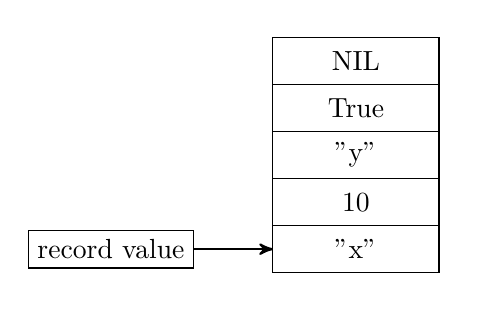
\begin{tikzpicture}

  \matrix (record) [matrix of nodes
    , nodes={ minimum height = 1.7em
            , minimum width = 6em
            , outer sep = 0pt
            , anchor = north
            , draw
            }
    , column sep=-\pgflinewidth % collapse borders
    , row sep=-\pgflinewidth % collapse borders
    , nodes in empty cells]
  {
    NIL   \\
    True  \\
    "y"   \\
    10    \\
    |(x)| "x" \\
  };

  \node (value) [left = of x,draw] {record value};

  \draw [-stealth',thick] (value.east) to [out=0,in=180] (x.west);

\end{tikzpicture}
\end{center}
\caption{Layout of a record value in memory.}
\label{fig_recordLayout}
\end{figure}

The code generator converts field names to 32-bit integers by numbering them,
starting by 1, in the order in which they are encountered during code
generation.  If a program uses more than $2^{32}-2$ different field labels,
compilation aborts with an error.  The number 0 is reserved for the sentinel
that marks the end of a record.  From now on, the term \emph{label}, when
used in the context of record implementation, refers to this number.

Record projection is implemented as a function of two arguments: the
pointer to a record and the label whose value to look up.  The lookup function
searches the record for a field whose label matches the given label, and returns
the associated value.  If lookup reaches the sentinel, the whole program
terminates, the idea being that the type checker prevents this from happening.
We still include this safety belt as good engineering practice.

\subsection{Subtyping of records}

\subsection{Type checking of records}


\section{Further work}

There are a few open points in the current implementation.

\begin{itemize}

  \item All identifiers are tracked in the same environment.  Therefore, the
  type checker doesn't forbid assignments to identifiers which refer to
  functions, or even built-in functions.

  \item There are no warnings or errors when name clashes occur.  The previously
  defined identifier is silently shadowed.

  \item Requiring the programmer to explicitly separate blocks of declarations
  could be automated by a dependency analysis.

\end{itemize}


\section{Examples}

This section describes the example programs which accompany this document.

\subsection{Examples for phase 1}

This section contains the compilation results for the provided examples from the
first assignment.  One of them had to be slightly modified, because it contained
non-capitalized boolen constants \texttt{true} and \texttt{false} instead of
\texttt{True} and \texttt{False}.

When parsing or type checking fails, the compiler prints an error message
indicating the cause of the error.  When both these phases succeed, the compiler
prettyprints the program, with inferred types instead of type annotations.

Function types in error messages are pretty-printed as a space separated list
of the argument types, followed by an arrow symbol, followed by the return
type.  For example, the type of the constant function is printed as \texttt{(a
b -> a)}, and the type of the main function as \texttt{( -> Void)}.

\begin{verbatim}
$ ./spl --typecheck -i examples/p1-examplePrograms/arguments.spl
"Couldn't match expected type `(Int Bool [Int] -> [Int])' with actual type `( -> a)' at position 15:5"

$ ./spl --typecheck -i examples/p1-examplePrograms/x.spl

// xMarksTheSpot : forall <3>, (<3> -> <3>)
a xMarksTheSpot(a x)
{
  return x;
}



$ ./spl --typecheck -i examples/p1-examplePrograms/Fib.spl

// fib : (Int -> Int)
Int fib(Int n)
{
  if( (n < 2) )
    return 1;
  else
    return (fib((n - 1)) + fib((n - 2)));
}



$ ./spl --typecheck -i examples/p1-examplePrograms/2D.spl

// foo : (Int -> (Int, Int))
(Int, Int) foo(Int n)
{
  return (2, 2);
}


// transpose : ((Int, Int) (Int, Int) -> (Int, Int))
(Int, Int) transpose((Int, Int) p1, (Int, Int) p2)
{
  return ((fst(p1) + fst(p2)), (snd(p1) + snd(p2)));
}


// scale : ((Int, Int) Int -> (Int, Int))
(Int, Int) scale((Int, Int) p, Int scalar)
{
  return ((fst(p) * scalar), (snd(p) * scalar));
}



$ ./spl --typecheck -i examples/p1-examplePrograms/Example.spl
"Couldn't match expected type `[Int]' with actual type `(a -> Int)' at position 21:55"

$ ./spl --typecheck -i examples/p1-examplePrograms/whitespaces.spl

// CAPPS : (Int Bool -> Void)
Void CAPPS(Int X, Bool S)
{
  X = 0;
  S = True;
  return;
}


// tabbed : ( -> Void)
Void tabbed()
{
  return;
}



$ ./spl --typecheck -i examples/p1-examplePrograms/lists.spl

// reverse : forall <3>, ([<3>] -> [<3>])
[a] reverse([a] list)
{
  // accu : [<3>]
  [a] accu = [];
  while( !isEmpty(list) )
  {
    accu = (head(list) : accu);
    list = tail(list);
  }
  return accu;
}


// sum : ([Int] -> Int)
Int sum([Int] list)
{
  return (head(list) + sum(tail(list)));
}


// product : ([Int] -> Int)
Int product([Int] list)
{
  return (head(list) * product(tail(list)));
}


// main : ( -> Void)
Void main()
{
  // list : [Int]
  [Int] list = (1 : (3 : (5 : [])));
  print(sum(list));
  print(product(list));
}



$ ./spl --typecheck -i examples/p1-examplePrograms/stress.spl
Failed parsing 'examples/p1-examplePrograms/stress.spl' :
Expected  at position LineColPos 10 1 367 expecting one of [Comment, Whitespace, "return", Identifier, Identifier, "while", "if", "{", "}"] at 11:2 :
                              v
rse as (!1):2, not !(1:2) */  [([foo],bar)] y = this_is_fine((1,(2,3)))
                              ^



$ ./spl --typecheck -i examples/p1-examplePrograms/SumProduct.spl

// sum : ([Int] -> Int)
Int sum([Int] list)
{
  if( isEmpty(list) )
    return 0;
  else
  {
  }
  return (head(list) + sum(tail(list)));
}


// product : ([Int] -> Int)
Int product([Int] list)
{
  if( isEmpty(list) )
    return 1;
  else
  {
  }
  return (head(list) * sum(tail(list)));
}


// sum : ([Bool] -> Bool)
Bool sum([Bool] list)
{
  if( isEmpty(list) )
    return False;
  else
  {
  }
  return (head(list) || sum(tail(list)));
}


// product : ([Bool] -> Bool)
Bool product([Bool] list)
{
  if( isEmpty(list) )
    return True;
  else
  {
  }
  return (head(list) && sum(tail(list)));
}



$ ./spl --typecheck -i examples/p1-examplePrograms/problematic_programs.spl
"Couldn't match expected type `(Int Int -> Int)' with actual type `(a b -> Void)' at position 8:53"

$ ./spl --typecheck -i examples/p1-examplePrograms/factorial.spl
"Unknown identifier `facL' at position 33:36"

$ ./spl --typecheck -i examples/p1-examplePrograms/booleans.spl
"Unknown identifier `null' at position 10:19"

$ ./spl --typecheck -i examples/p1-examplePrograms/pass_nested_expr.spl

// main : ( -> Int)
Int main()
{
  return 5;
}



$ ./spl --typecheck -i examples/p1-examplePrograms/empty.spl
Failed parsing 'examples/p1-examplePrograms/empty.spl' :
Expected  at position LineColPos 5 0 122 expecting one of [Comment, Whitespace, "[", "(", Identifier, "return", Identifier, Identifier, "while", "if", "{"] at 6:1 :
                              v
rseerd worden. Void main () { }  
                              ^



$ ./spl --typecheck -i examples/p1-examplePrograms/problematic.spl
"Couldn't match expected type `Int' with actual type `( -> Int)' at position 10:16"

$ ./spl --typecheck -i examples/p1-examplePrograms/3D.spl
"Unknown identifier `first' at position 3:32"

$ ./spl --typecheck -i examples/p1-examplePrograms/example10.spl
"Unknown identifier `null' at position 10:16"

$ ./spl --typecheck -i examples/p1-examplePrograms/list.spl

// equals : ([Int] [Int] -> Bool)
Bool equals([Int] a, [Int] b)
{
  if( (isEmpty(a) && isEmpty(b)) )
    return True;
  else
  {
  }
  if( (isEmpty(a) || isEmpty(b)) )
    return False;
  else
  {
  }
  return ((head(a) == head(b)) && equals(tail(a), tail(b)));
}



$ ./spl --typecheck -i examples/p1-examplePrograms/while.spl

// keepGoingI : (Int -> Void)
Void keepGoingI(Int n)
{
  while( True )
  {
    n = (n + 1);
  }
}


// keepGoingR : (Int -> Void)
Void keepGoingR(Int n)
{
  return keepGoingR((n + 1));
}



$ ./spl --typecheck -i examples/p1-examplePrograms/op.spl
// n : Int
Int n = 5;

// op : Bool
Bool op = (((1 + (n / 2)) - (n % 2)) < n);

// op2 : Bool
Bool op2 = ((((1 + n) / 2) - (n % 2)) < n);



$ ./spl --typecheck -i examples/p1-examplePrograms/sum.spl
Failed parsing 'examples/p1-examplePrograms/sum.spl' :
Expected  at position LineColPos 25 13 346 expecting one of [Comment, Whitespace, "]"] at 26:14 :
                              v
}  Void main() {  print (sum([1:2:3:[]]));  print (sum1([1:2:3:[]]));  
                              ^



$ ./spl --typecheck -i examples/p1-examplePrograms/integers.spl

// abs : (Int -> Int)
Int abs(Int n)
{
  if( (n < 0) )
    return -n;
  else
    return n;
}



$ ./spl --typecheck -i examples/p1-examplePrograms/bool.spl

// xor : (Bool Bool -> Bool)
Bool xor(Bool a, Bool b)
{
  return ((a || b) && !(a && b));
}


// implies : (Bool Bool -> Bool)
Bool implies(Bool a, Bool b)
{
  if( !a )
    return True;
  else
    return b;
}



$ ./spl --typecheck -i examples/p1-examplePrograms/mergeSort.spl
"Unknown identifier `split' at position 20:20"

$ ./spl --typecheck -i examples/p1-examplePrograms/mklinik.spl

// foobar : ( -> Int)
Int foobar()
{
  return -10;
}
\end{verbatim}

\subsection{Examples for phase 2}

This section contains descriptions for the example programs for phase 2 which
accompany this document.  Each example is given in an .spl file, and the output
of the compiler is given in a .txt file with the same filename.

\begin{description}

  \item[pass-fold-map.spl] Higher-order functions usually found in functional
  programming: \emph{foldl}, \emph{foldr}, \emph{map} and \emph{filter}.

  \item[pass-mutual-recursion.spl] Two mutually recursive functions. The
  arguments are flipped in the recursive calls, constraining their types to $(a
  \arr a \arr b)$.

  \item[fail-mutual-recursion-lists.spl] Mutually recursive values are not
  allowed.

  \item[pass-polymorphism-mutual-recursion.spl] The polymorphic identity can be
  instantiated differently in two mutually recursive functions.  This works
  because $f$ and $g$ are marked to be unified together, but independently of
  \emph{id}.  Putting the braces around all \emph{id}, $f$ and $g$ gives a type
  error.  See fail-polymorphism-mutual-recursion.spl

  \item[fail-polymorphism-mutual-recursion.spl] The polymorphic identity cannot
  be instantiated differently in two mutually recursive functions.  That is
  because the types of all three functions are unified simultaneously.

  \item[pass-transitive-locals-backwards.spl] The return type of the function
  constrains all local variables to be of type $\text{Int}$, which constrains
  the function argument to be also of type $\text{Int}$.

  \item[fail-unknown-identifier.spl] Demonstrates the error message given when
  an undefined identifier occurs in a program.

  \item[fail-not-enough-function-arguments.spl] Demonstrates the error message
  given when a function is called with too few arguments.

  \item[fail-no-polymorphism-in-variables-lvalues.spl] Assigning to a global
  variable constrains its type, even if it is initialized with a polymorphic
  value.  Therefore, it is forbidden to assign values of different types to a
  global variable.

  \item[fail-no-polymorphism-in-variables-rvalues.spl] Using a global variable
  in an expression constrains its type, even if it could be polymorphic.  This
  is the tradeoff we had to make for assignments to be sound.

  \item[pass-assignment-to-function.spl] It is possible to bind functions to
  local variables, assign to them, and call them.

  \item[shouldfail-assignment-to-function.spl] It should be forbidden to assign
  to identifiers which are bound to global functions.  To be done.

  \item[pass-return-function.spl] A function can return another function.

  \item[fail-return-function.spl] It is not possible to directly call the return
  value of a function that returns another function.

  \item[pass-assign-global-to-argument.spl] Function $f$ assigns its first
  argument, $y$, to the global $x$.  This ties their types together, and as a
  result the type of $y$ is not generalized.  The concrete type of $y$ is
  determined by the first occurrence where $f$ is used.  Here, $f$ is of type:
  $\forall a . ([\text{Int}] \arr a \arr a)$.

  \item[pass-assign-argument-to-global.spl] The same as
  pass-assign-global-to-argument, but this time it's the argument that is
  assigned to.

\end{description}

\subsection{Examples for phase 3}
\label{sec_examplesPhase3}

This section contains descriptions for the example programs for phase 3 which
accompany this document.  Each example is given in an .spl file, together with
an .ssm file which contains the generated code.  The \emph{print} function
prints its argument as an integer, followed by a newline.  The output of the
program is given here, with newlines replaced by spaces.

\begin{description}

  \item[access-variables.spl] Read- and write local and global variables and
  function arguments. Output:

  \begin{verbatim}
  1 2 3 2 4 6
  \end{verbatim}

  \item[logical-operators.spl] Implements logical implication and equivalence in
  terms of \emph{not}, \emph{and} and \emph{or}. Output:

  \begin{verbatim}
  -1 -1 0 -1 -1 0 0 -1
  \end{verbatim}

  \item[recursion-iteration.spl] Recursive and iterative variants of the
  fibonacci function. Demonstrates recursive function calls and while loops.
  Output:

  \begin{verbatim}
  1 89 10946 1 89 10946
  \end{verbatim}

  \item[gcd.spl] Calculates the greatest common divisor using Euclid's
  algorithm. Output:

  \begin{verbatim}
  1 21 21
  \end{verbatim}

  \item[lists.spl] Calculates a list of fibonacci numbers.  Demonstrates list
  construction and destruction. Output:

  \begin{verbatim}
  10946 6765 4181
  \end{verbatim}

  \item[map-filter.spl] Higher-order functions map and filter. Output:
  \begin{verbatim}
  1 4 6
  \end{verbatim}

  \item[function-return-value.spl] Functions as return values of functions.
  Output:
  \begin{verbatim}
  8 -2
  \end{verbatim}

  \item[uninitialized-variable.spl] Magically pass a value from one function
  call to another by using the implementation detail that local variables occupy
  the same position on the stack. Output:

  \begin{verbatim}
  42 100
  \end{verbatim}

  \item[list-of-tuples.spl] The function \emph{zip} turns a tuple of lists into
  a list of tuples, while \emph{unzip} does the opposite. Output:

  \begin{verbatim}
  4 3 3 100
  \end{verbatim}

  \item[mutual-recursion.spl] A complicated way to add two numbers. Output:

  \begin{verbatim}
  8 10 20
  \end{verbatim}

\end{description}


\bibliographystyle{plain}
\bibliography{computer_science}

\end{document}

% vim: textwidth=80
